\documentclass[preprint,NumberedRefs]{JASA}
\DeclareMathOperator*{\argmin}{argmin}


\begin{document}

\title[Transverse-longitudinal reconstruction]{Reconstruction of transverse-longitudinal vibrations in the organ of Corti complex via optical coherence tomography}
\author{Brian L. Frost}
\affiliation{Department of Electrical Engineering, Columbia University, 500 W. 120th St., Mudd 1310, New York, NY 1002, USA.}
\email{b.frost@columbia.edu}
\author{Clark Elliott Strimbu}
\affiliation{Department of Otolaryngolgy Head and Neck Surgery, Vagelos College of Physicians and Surgeons, Columbia University, 630 W 168th St, New York, NY 10032.}
\author{Elizabeth S. Olson}
\affiliation{Department Biomedical Engineering, Columbia University, 351 Engineering Terrace, 1210 Amsterdam Avenue,New York, NY 10027. Also at Department of Otolaryngolgy Head and Neck Surgery.}

\preprint{Frost, JASA}

\date{\today} 


\begin{abstract}

\end{abstract}


\maketitle

\section{Introduction}
\par{Optical coherence tomography (OCT) is a powerful instrument for the study of cochlear mechanics. It is capable both of volumetric imaging and sub-nanometer vibrometry at a depth into a sample \citep{OCTtheory,sdpm}, allowing for the measurement of motion inside of the organ of Corti complex (OCC) \textit{in vivo} \citep{gao,dongoghalai,fallah,strimbu2020,fangyi,lee,cooper}. These data have provide significant insight into OCC micromechanics, both improving our understanding of and raising many questions about the mechanisms responsible for the incredible dynamic range of the sensitive cochlea. However, certain limitations of OCT can greatly complicate the interpretation of these data.}
\par{OCT vibration measurements and images are built from one-dimensional axial scans (A-Scans), generated via the Fourier transform of raw photodetector data. The magnitude of the A-Scan indicates the reflectivity at different depths into the sample. Images (referred to as brightness scans, or B-Scans) are built by taking a series of A-Scans along a line perpendicular to the optical axis. Many parallel B-Scans can be taken to form a volume scan.}
\par{A series of A-Scans at one location is referred to as a motion scan (M-Scan). The phase of a single pixel as a function of time is proportional to the sub-pixel displacement \textit{along the axis of the beam} of structures at that position \citep{sdpm}. That is, an M-Scan allows us to measure a projection of the 3-D motion of a structure onto the beam axis.}
\par{The nature of the modality leads to several important complications: (1) as OCT images are based on reflectivity, they are \textit{label-free}, so structures must be identified via known anatomy and intuition; (2) displacement measurements are 1-D projections of 3-D motions. These issues are even further complicated by the fact that the optical axis is often decided via the constraints of the preparation, and its relationship to the anatomy is often not known \textit{a priori}.}
\par{We have discussed these issues in terms of the anatomical coordinates of the cochlea (longitudinal, radial and transverse), using volume scans to determine the optical axis' relation to more physiologically relevant axes \citep{frost2022}. Using this method, one can account for the longitudinal (tonotopic) distance between measured points in a single A-Scan. One can also determine which components of motion are most represented in a measurement, offering more context to reported results. However, even this is not sufficient to separate out the motion components themselves.}
\par{It has been shown by Cooper et al that viewing angle can significantly impact both the magnitude and phase response of the structures being measured \citep{cooper2018}. For example, purely transverse measurements in the gerbil base have shown different character than measurements taken at an angle relative to basilar membrane (BM) normal \citep{Puria2022}. SHOW SOME FIGURE HERE FOR DIFFERENCES.}
\par{Recent efforts have been made to better understand intra-OCC motion at anatomically relevant angles, as these measurements could better aid in our understanding of cochlear micromechanics. For example, radial motion of the tectorial mebrane and stereocilia is responsible for the transduction that results in neural responses and electromotility in inner and outer hair cells, respectively. Longitudinal motion may clarify the impact of fluid motion intra-OCC, where cells may not simply move as rigid bodies.} 
\par{One possible solution is to measure motion directly at an angle of interest. For example, Cho et al have measured at a transverse angle in the hook region of the gerbil base, and Ren et al have similarly made purely transverse measurements of the reticular lamina in the gerbil base. Preliminary work has also been done to make exclusively radial measurements of intra-OCC motion in mouse. However, such measurement angles are not available in certain preparations, dependent on species and frequency location of interest.}
\par{Other methods have been developed to reconstruct motion along physiologically relevant axes without directly measuring along any of these axes explicitly. Lee et al used back-projection of measurements taken at two different angles to reconstruct radial-transverse motion in mouse, via carefully rotating the preparation to ensure they stay in the same cross-section \citep{lee}. Kim et al used a three-beam OCT system in mouse to measure motion at the same location from three angles, and back-project to resolve three-dimensional motion CITE. These methods are challenging to implement in the gerbil base, where the anatomy and opacity of the bone significantly restricts the beam angle when viewing through the round window (RW). The latter method also requires significant hardware and space.}
\par{We have developed a method to reconstruct the longitudinal and transverse components of motion \textit{in vivo} via OCT. Similar to the work described above, we reconstruct via back-projecting measurements taken at two angles. However, our method performs registration via \textit{physiology} rather than mechanical precision -- our method requires no \textit{a priori} knowledge of either measurement angle, or of the precise positions of the structures being measured. Instead we use the traveling wave phase on the BM, along with a simplified version of the orientation program presented in Frost et al, 2022, to register intra-OCC positions between viewing angles. This allows the method to work in any species or preparation, including in the gerbil base in which we are particularly interested.}
\par{We present the method, an analysis of the accuracy of this method as a function of angular distance between viewing angles, and \textit{in vivo} experimental data taken through the RW in gerbil. We present longitudinal and transverse motion at the outer hair cell/Deiters' cell junction (OHC-DC), and see that the transverse data matches well with previously measured purely transverse motion in the gerbil base. In particular, we see that transverse OHC-DC motion phase lags BM motion phase across frequency by ~0.3 cycles, save at high SPL where the two seem to move in-phase. This is in stark contrast with motion measured at an angle with a longitudinal component, where a broadband phase lead of OHC-DC re BM is often seen \citep{frost2022}.}

\section{Methods}
\par{In this section, we will present our method for reconstructing transverse-longitudinal motion in the OCC. To begin, we will present the mathematical basis for this method. Then, we will describe the experimental process by which the quantities required for the reconstruction are acquired.}
\subsection{Mathematics of reconstruction}
\par{The true motion of each structure is three-dimensional. However, in this work, we are only concerned with longitudinal and transverse motion components. Ensuring that our measurement angles have no radial component, we can consider the ``true motion" of a single point of interest as being a two-dimensional vector. Call the longitudinal and transverse unit vectors $\mathbf{\hat{l}}$ and $\mathbf{\hat{t}}$, respectively. The true displacement can be written as a two-vector with longitudinal and transverse components as 
\begin{equation}
    \mathbf{d} = d_l \mathbf{\hat{l}} + d_t \mathbf{\hat{t}}.
\end{equation}
}
\par{Our beam axis is a unit vector that can also be written in anatomical coordinates, having a transverse and longitudinal component. Consider two such beam axes,
\begin{equation}
    \mathbf{z}_1 = l_1 \mathbf{\hat{l}} + t_1 \mathbf{\hat{t}},\;\;\mathbf{z}_2 = l_2 \mathbf{\hat{l}} + t_2 \mathbf{\hat{t}}.
\end{equation}
}
\par{We take measurements of the point of interest along both of these axes, $\delta_1$ and $\delta_2$. These are 1-D displacements, defined as the projection of the true motion $\mathbf{d}$ onto $\mathbf{z}_1$ and $\mathbf{z}_2$, respectively. Mathematically, this relationship is described as a dot product: 
\begin{equation}
	\delta_i = \mathbf{z}_i^T\mathbf{d},\;i=1,2.
\end{equation}
We can also write this as a system of two equations in matrix form as
\renewcommand*{\arraystretch}{.5}
\begin{equation}
	\begin{pmatrix}\delta_1\\ \delta_2\end{pmatrix} = \begin{pmatrix}l_1&t_1\\l_2&t_2\end{pmatrix}\begin{pmatrix}d_l\\d_t\end{pmatrix},
\end{equation}
or to solve for $\mathbf{d}$,
\renewcommand*{\arraystretch}{.5}
\begin{equation}
	\begin{pmatrix}d_l\\d_t\end{pmatrix}= \begin{pmatrix}l_1&t_1\\l_2&t_2\end{pmatrix}^{-1}\begin{pmatrix}\delta_1\\ \delta_2\end{pmatrix}.
		\label{recon}
\end{equation}
}
\par{Our goal is to reconstruct the 2-D motion, i.e. to find $\mathbf{d}$. To solve for $\mathbf{d}$, we need to measure $\delta_1$ and $\delta_2$ \textit{at the same location}, and we need to find anatomical coordinate representations of the measurement axes (i.e. the elements of the $2\times 2$ matrix in Eq. \ref{recon}).}
\subsection{Experimental method}
\par{To perform the reconstruction according to Eq. \ref{recon}, we must be able to (1) determine the measurement axes in anatomical coordinates ($l_i$ and $t_i$), and (2) register a point of interest between two orientations so that the \textit{same structure} may be measured at both angles. We present a method that performs both of these tasks without any \textit{a priori} knowledge of precise location structures or beam angles, using only a single OCT system and the traveling wave physiology of the mammallian cochlea. Each step is also presented visually in a panel in FIGURE.}
\par{We begin with our OCT system viewing the OCC at some unknown angle with respect to the BM normal. Using the ThorLabs ThorImage software, we are able to view a real-time volume scan of the sample at this angle. Doing so, we note two points in the volume which lie on the same anatomical structure, and refer to their 3-D coordinates as $\mathbf{p}_1$ and $\mathbf{p}_2$. For example, $\mathbf{p}_1$ could be chosen to lie at the OHC-DC junction in some cross-section, and $\mathbf{p}_2$ to lie at the OHC-DC junction in a different cross-section. Note that these points are specified in \textit{optical} coordinates, where $\mathbf{\hat{z}}$ is the optic axis (depth), and $\mathbf{\hat{x}}$ and $\mathbf{\hat{y}}$ are the scanning directions.}
\par{While the longitudinal and transverse directions are not constant in space -- they change along with the spiral of the cochlea -- one can approximate them as being stationary. This amounts to the local approximation of the BM as a plane, which is reasonable over a range of $\sim 200$ $\mu$m \citep{frost2022}. Wehn approximated this way, the line segment connecting anatomical structures of the same type between cross-sections is parallel to the longitudinal axis. That is, the longitudinal unit vector is given in optical coordinates by
\begin{equation}
	\mathbf{\hat{l}} = \frac{\mathbf{p}_2-\mathbf{p}_1}{||\mathbf{p}_2-\mathbf{p}_1||}.
\end{equation}
The component of the measurement axis in the longitudinal direction is simply the $\mathbf{z}$ component of $\mathbf{\hat{l}}$. That is, at each angle $i=1,2$, the longitudinal component is
\begin{equation}
	l_i = \mathbf{\hat{l}}\cdot\mathbf{z}.
\end{equation}
}
\par{Next we recall that the measurement axis $\mathbf{z}_i$ is a \textit{unit} vector, so $t_i^2 + l_i^2 = 1$. This means that
	\begin{equation}
		t_i = \sqrt{1-l_i^2}.
	\end{equation}
	With this, we have now found the elements of the matrix in Eqn \ref{recon}. The next goal is to register points to one another between orientations.
}
\par{For reasons we will motivate shortly, we begin by taking many measurements of the structure of interest along the longitudinal axis. For example, at orientation $i=1,2$, if we are interested in the OHC-DC, we find a single point in this region and call it $\mathbf{q}_0$. By the definition of the longitudinal direction, for any real $a$, $\mathbf{q}_0 + a\mathbf{\hat{l}}$ is also in the OHC-DC region. We choose a number of points $N$ and a spacing $\delta$ and take measurements at points
	\begin{equation}
		\mathbf{q}^i_n = \mathbf{q}^i_0 + n\delta\mathbf{\hat{l}},\;n=0,1,\ldots,N.
	\end{equation}
}
\par{This gives us $N$ measurements of the structure evenly spaced longitudinally. In each measurement line, we inevitably also measure BM at some point $\mathbf{b}^i_n$. As $\mathbf{z}\neq\mathbf{\hat{t}}$, the OHC-DC and BM points measured in each line are not in the same longitudinal cross-section. For example, suppose that on the $\mathbf{z}$ axis in a single A-Scan, the BM and OHC-DC are $\Delta = (\mathbf{p}^i_n-\mathbf{b}^i_n)\cdot\mathbf{z}$ apart. Ideally, this value is independent of the cross-section, or $n$. The cross-sectional distance (i.e. longitudinal distance) between these points is thereby $r^i = \Delta l_i$.}
\par{Now let's once again consider our first OHC-DC measurement at $\mathbf{q}^i_0$. It is in the same cross-section as a point on the BM at $\mathbf{b}^i_0+r^i\mathbf{\hat{l}}$. We have taken many measurements of BM along the longitudinal axis, so if $\delta$ is small, there exists an $n$ such that $r^i \approx n\delta$. That is, $\mathbf{q}^i_0$ is approximately in the same cross-section as $\mathbf{b}^i_n$ for this $n$.}
\par{We can repeat this process for all measured OHC-DC points to form a list of \textit{aligned} OHC-DC/BM pairs (i.e. OHC-DC and BM in the same cross-section) at each orientation. Using this list, we can reformulate the problem of registering OHC-DC points as one of registering BM points -- the OHC-DC points aligned to these BM points would also be registered.}
\par{To register BM points between orientations, we use the traveling wave to our advantage. To begin, \textbf{we assume that the BM moves entirely transversely}. This means that viewed at any angle, the phase response of BM motion will be identical. To register points on the BM between orientations, we compare the phase response at $\mathbf{b}^1_n$ to $\mathbf{b}^2_m$ for $n,m=1,2,\ldots,N$, and find the values for which the phase responses are most similar by minimum $L_2$ distance.}
\par{That is, we start by comparing the phase response at $\mathbf{b}^1_0$ to $\mathbf{b}^2_m$ for $m=0,1,\ldots,N$, $\phi^1_0(f)$ and $\phi^2_m(f)$ respectively where $f$ is frequency. We find 
	\begin{equation}
		m_0 = \argmin_m E_{0,m} = \argmin_m ||\phi^1_0(f)-\phi^2_m(f)||,
	\end{equation}
and consider $\mathbf{b}^1_0$ and $\mathbf{b}^2_{m_0}$ to be registered. Because BM positions measured are spaced evenly longitudinally by $\delta$ in either orientation, this means that $\mathbf{b}^1_1$ and $\mathbf{b}^2_{m_0+1}$ are also registered, and so on.}
\par{This yields registered BM points across some range of the BM. As we aligned the BM points to OHC points in the previous step, we now have OHC-DC points registered as well. We can then perform our reconstruction.}
\par{To make this process more concrete, we provide an illustrative example in the Results section below.}
\subsection{Error dependence on angular difference}
\par{The presentation above is in an ideal environment, wherein the reconstruction can be performed from any two measurements at distinct angles. Mathematically, the error associated with the angular difference arises from the matrix in Eqn \ref{recon}. Note that this matrix must be invertible, which require full row rank -- i.e. the rows must not be colinear. The rows of this matrix are the measurement axes, $\mathbf{z}_1$ and $\mathbf{z}_2$, which will never be colinear by design. The invertibility of this matrix is thereby guaranteed.}
\par{However, it is intuitively clear that reconstructions could not be reliably made from two measurements taken, say, 1$^\circ$ apart. This lies in the fact that the matrix has a multiplicative impact on the noise in measurements $\delta_1$ and $\delta_2$. As a rule of thumb, if $\sigma_{max}$ and $\sigma_{min}$ are the maximum and minimum singular values of a matrix, then matrix multiplication reduces the SNR by a factor of the \textit{condition number}:}
\begin{equation}
	\kappa = \frac{|\sigma_{max}|}{|\sigma_{min}|}.
\end{equation}
\par{It can be shown that a matrix and its inverse have the same condition number. The formula for the singular values of a $2\times2$ matrix (using the element names of the relevant matrix) is known to be
	\begin{align}
		\sigma_{max} &= \sqrt{\frac{s_1+s_2}{2}},\\
		\sigma_{min} &= \sqrt{\frac{s_1-s_2}{2}},
	\end{align}
where
	\begin{align}
		s_1 &= l_1^2 + t_1^2 + l_2^2 + t_2^2,\\
		s_2 &= \sqrt{(l_1^2 + t_1^2 - l_2^2 - t_2^2) + 4(l_1l_2 + t_1t_2)^2}.
	\end{align}
}
\par{We know that the measurement axes are unit vectors, so $l_i^2+t_i^2 = 1$ for $i=1,2$. That gives $s_1 = 2$ and $s_2 = 2(l_1l_2 + t_1t_2)$. Defining $\nu = l_1l_2+t_1t_2$, we simplify condition number formula to
	\begin{equation}
		\kappa = \sqrt{\frac{1+\nu}{1-\nu}},
	\end{equation}
a monotonically increasing function of $\nu$.
}
\par{We now note that $\nu = \mathbf{z}_1\cdot\mathbf{z}_2$, whichmay offer a bit of intuition -- the dot product is largest when the two vetors are nearer to parrallel, yielding an increase in condition number. To be more mathematically precise,
	\begin{equation}
		\nu = ||\mathbf{z}_1||\,||\mathbf{z}_2||\cos{\theta} = \cos{\theta},
	\end{equation}
where $\theta$ is the angular distance between the two vectors and we have used the fact that the measurement axes are unit vectors. We now can use double angle trigonometric identities to write the condition number very succinctly as a function of the angular difference between the two measurement axes:
	\begin{align}
		\kappa &= \sqrt{\frac{1+\cos\theta}{1-\cos\theta}}\\
			   &=\sqrt{\frac{1}{\tan^2\frac{\theta}{2}}}\\
			   &=\frac{1}{\big|\tan\frac{\theta}{2}\big|}.
	\end{align}
}
\par{The condition number goes to infinity when the angular difference approaches 0, and approaches a minimum at 1 as the angular difference approaches 90$^\circ$. While 90$^\circ$ would be optimal, the maximum achievable angular difference is restricted by the experimental preparation. For example, in measurements taken through the gerbil round window, 15$^\circ$ is often the largest achievable angular difference. Table \ref{kappas} shows condition numbers for a selection of angular deviations achievable in gerbil through the round window membrane.}
\par{For context, the noise floor of our displacement measurements is approximately 0.1 nm. For a vector of two independent measurements $\delta_1$ and $\delta_2$, our noise floor would thereby be about $\sqrt{0.1^2 + 0.1^2}\approx0.14$ nm. The noise increase induced by reconstruction using measurements taken 15$^\circ$ (a factor of 7.6, according to Table \ref{kappas}) apart would yield a noise floor of $\sim$1 nm.}

\begin{table}
\begin{center}
	\begin{tabular}{|c|c|}
        \hline
        Angular deviation & Condition number $\kappa$ \\
        \hline
		20$^\text{o}$ & 5.67\\
        15$^\text{o}$ & 7.60\\
        10$^\text{o}$ & 11.43\\
        5$^\text{o}$ & 22.90 \\
        1$^\text{o}$ & 114.59\\
        \hline
    \end{tabular}
    \caption{A table of condition numbers for the projection matrix at possible measurement angular deviations.}
\label{kappas}
\end{center}
\end{table}

\par{\section{Results}
We begin with an illustrative example of the method in an \textit{in vivo} gerbil preparation, wherein measurements were taken through the RW. The measurements are then compared to previously measured purely transverse OCC displacements.}
\subsection{Illustrative example}
\par{We choose to take $N=11$ measurements at each orientation of the sample, spaced $\delta=15$ $\mu$m apart longitudinally. Viewing the sample at the first orientation, we choose two points at the OHC-DC location,$\mathbf{p}^1_1$ and $\mathbf{p}^1_2$, and take their difference to find the longitudinal axis $\hat{l}^1=(,,)^T$. We choose $\mathbf{q}^1_0=\mathbf{p}^1_1$, as we are interested in points at the OHC-DC region. We then take 11 measurements, at $\mathbf{q}^1_0,\mathbf{q}^1_0+15\mathbf{\hat{l}}^1,\ldots,\mathbf{q}^1_0+(11\times15)\mathbf{\hat{l}}^1$.Our measurements are made using a 15-frequency Zwuis tone stimulus at several 40, 50, 60, 70 and 80 dB SPL.}
\par{We repeat this process at the second orientation, where we find $\mathbf{\hat{l}}^2=(,,)^T$. This gives us all of the measurements we need for the experiment as described in the Methods section, and we can proceed with the mathematical reconstruction.}
\par{The $\mathbf{\hat{z}}^i$-components of the unit longitudinal vectors let us find the measurement matrix components from Eqn \ref{recon}:
	\begin{align}
		l_1 = &,\;t_1 = \sqrt{1-l_1^2}= \\
		l_2 = &,\;t_2 = \sqrt{1-l_2^2}=.
	\end{align}
}
\par{Next, we look at A-Scans at each orientation to find aligned BM and OHC-DC points in the same cross-section. Considering an A-Scan taken at position $\mathbf{q}^1_0$, we see that the OHC-DC junction and BM measurements lie  pixels apart. In our system, a pixel is 2.7 $\mu$m, so the structures are longitudinally $\Delta = $ apart in the optical axis. This means that they lie $\Delta l_1 = $ apart longitudinally. Of all multiples of $\delta = 15$ $\mu$m, this value is closest to $ = \delta$. That is, this OHC-DC measurement is approximately aligned with the BM measured at $\mathbf{q}^1_0+\delta\mathbf{\hat{l}}=\mathbf{q}^1_2$. This BM point is $\mathbf{b}^1_2$, i.e. we have aligned OHC-DC $\mathbf{q}^1_0$ with BM $\mathbf{b}^1_2$.}
\par{This relation holds for the rest of the points measured at this angle, so that the OHC-DC points are generally three runs apart from BM measured in the same A-Scan. This means that OHC-DC $\mathbf{q}^1_1$ is in the same cross-section as BM $\mathbf{b}^1_3$, and so on up to OHC $\mathbf{q}^1_8$ is aligned to $\mathbf{b}^1_{11}$. We can do the same at the second orientation as well to align OHC-DC points and BM points.}
\par{Now we register BM points between orientations. We start by comparing the phase responses $\phi^1_0$ to $\phi^2_m$ for $m=0,1,\ldots,10$, and find that the BM from measurement 0 at orientation 1 is best aligned with BM from measurement   at orientation 2. This gives us several registered BM pairs, namely . An example of the matched phase responses can be seen in FIGURE, wherein the phase responses of BM points taken at these two orientations are nearly identical.}
\par{Taking the registered BM points and observing our list of aligned BM and OHC-DC points, we can register several OHC-DC points to one another, namely . We can now perform the mathematical reconstruction at these locations.}
\par{Reconstructions of longitudinal and transverse motion at the OHC-DC region at 4 positions alongside BM data from the same cross-section are shown in FIGURE. The features of these data are described below.}
\par{As a note, using the values of $l_1$, $t_1$, $l_2$ and $t_2$ found above, we see that our measurement axes made  and  angles with the BM normal at orientations 1 and 2, respectively. The angular difference,   , yields a measurement matrix with condition number  . This is the factor by which our noise level is increased as a result of our reconstruction.}
\subsection{Features of the data and comparison to previous measurements}
\par{Observing first the magnitude of the reconstructed data, we see that OHC-DC motion in both the longitudinal and transverse direction are tuned to the same frequency as the BM, although less sharply than BM. Both components also show broadband linearity, which is characteristic of past OHC measurements made using tone complex stimuli. Transverse and longitudinal components of motion have similar magnitude at lower SPL, but diverge at 80 dB SPL.}
\par{Observing the phase, the transverse component of OHC-DC motion at SPL lower than 80 dB lags BM across frequency by $\sim 0.3-0.4$ cycles. At 80 dB SPL and near the best frequency, the OHC-DC transverse component and BM move in phase. The longitudinal component is approximately half a cycle out of phase from transverse displacement across much of the tested frequency range. By the definition of our axes, this means that base-to-apex motion is approximately in phase with Scala Media-to-Scala Tympani motion.}
\par{To validate our method, we compare to previously measured transverse data. Recent measures from Cho et al and our lab from the hook region are shown in FIGURE. Cho et al's measurements are taken using single-tone stimuli, while ours are taken using Zwuis tone complexes. Comparing to our reconstruction, we can see the following about OHC-DC transverse motion: 1) the motion exhibits broadband nonlinearity when measured using Zwuis tone complexes; 2) it is tuned to the same frequency as BM; 3) at frequencies above 0.5 BF, OHC-DC transverse phase lags BM by $\sim$0.3 cycles at lower SPL; 4) at higher SPL near BF, BM and OHC-DC move in phase in measurements taken using Zwuis tone complexes. }
\par{These characteristic similarities provide evidence that our model is correctly reconstructing these components of motion in the OHC-DC region. In particular, our original puzzle -- that OHC-DC re BM phase responses look vastly different when measured from different angles -- is resolved by these data.}
\par{Our reconstruction also indicates that there is a significant component of motion in the longitudinal direction at the OHC-DC junction. As the OHCs are not significantly longitudinally slanted in gerbil (CITE), this is not readily interpreted as a feature of electromotility. Instead, it may indicate the effects of fluid on these structures that is distinct from the more rigid BM, or the impact of other longitudinally tilted processes within the OCC (CITE) on OHC-DC. Study of longitudinal motion in other regions of the OCC could shed more light on the interpretation of measurements such as these.}
\section{Extensions of the method}
\par{Here we discuss two theoretical extensions of the method presented here -- one in which the accuracy of the method is improved by measuring from more than two longitudinal-transverse angles, and one in which the method is extended to reconstruct all three components of motion. Similar to the presented methods, these techniques require only a single OCT system and do not require any \textit{a priori} knowledge of the measurement angles or precise locations of the structures being measured.}
\par{Both proposed extensions require measurements at more than two angles to be taken. This would result in an improvement of the measured data, but would also be significantly more time-consuming and reduce the experiment's yield.}
\subsection{Overdetermined reconstruction}
\par{In the method presented above, we take measurements from two angles and solve a deterministic system of two linear equations in two variables. We note the impact of noise in these measurements as it pertains to the condition number of the measurement matrix, which can only be improved via increasing the angular difference between measurement angles.}
\par{However, one could also improve the accuracy by employing the same experimental method, but measure structures at $M>2$ angles. We call the measured displacements of a registered structure along these axes $\delta_1,\delta_2,\ldots,\delta_M$ and write the respective measurement axes in terms of components $l_1,t_1,l_2,t_2,\ldots,l_M,t_M$. At each registered location, one would now have a system of $M$ equations in 2 variables -- an overdetermined system. Mathematically, we can write the system as follows:
	\begin{equation}
		y=Ax
		\label{overd}
	\end{equation}
}
\par{As a result of noise, this over-determined system will not have a solution -- no value of the true motion $\mathbf{d}$ can yield all $M$ measured projections. Instead, we must make an \textit{educated guess} of the true motion based on our noisy projection measurements.}
\par{The equation \textit{actually} describing the projection at angle $m=1,2,\ldots,M$ is 
	\begin{equation}
		d_l l_m+d_t t_m + \eta_m = \delta_m,
	\end{equation}
where $\eta_m$ is a realization of noise that is different in each measurement, and of course, unknown. Thereby, instead of trying to solve this equation, we try to minimize:
\begin{equation}
	\mathcal{E}=\sum_{m=1}^M ||\delta_m-(d_ll_m + d_t t_m)||^2.
\end{equation}
The values of $d_l$ and $d_t$ that minimize $\mathcal{E}$ are the least-squares-optimal solution to this overdetermined problem.}
\par{In general, let $\mathbf{x}$ and $\mathbf{y}$ be vectors and $A$ be a matrix. The least-squares-optimal solution to an overdetermined linear system $\mathbf{y}=A\mathbf{x}$ is $\mathbf{x}_0=A^\dagger y$, where $A^\dagger$ is the \textit{Moore-Penrose pseudoinverse} of $A$. Most computational software packages include a routine to compute this pseudoinverse (for example, MATLAB's \texttt{pinv}.}
\par{If one wished to employ this version of the method, they would take measurements at $M$ angles along a large longitudinal stretch as described above. They would compute $l_m$ and $t_m$ for each orientation, and register points based on BM phase just as in the two-angle case. At each registered point, they will then reconstruct the true motion via
\begin{equation}
	\mathbf{d} = A^\dagger \delta.
\end{equation}
Note that as the pseudoinverse of an invertible matrix is equal to the inverse of said matrix, this equation degenerates to Eqn \ref{recon} from the standard method in the $M=2$ case.
}

\subsection{Extension to three dimensions}
\par{Naturally, after two-dimensional reconstruction, one looks to the third and final spatial dimension -- in this case, the radial dimension. To reconstruct three-dimensional motion requires motion measurements from three angles, and also requires at least one of our measurement axes to have a radial component. This complicates certain steps in our experimental method, but not insurmountably so.}
\par{First, let's note the 3-D reconstruction formula as a simple generalization of the 2-D formula:
\renewcommand*{\arraystretch}{.5}
	\begin{equation}
		\begin{pmatrix}d_l\\d_r\\d_t\end{pmatrix} = \begin{pmatrix}l_1&r_1&t_1\\l_2&r_2&t_2\\l_3&r_3&t_3\end{pmatrix}^{-1}\begin{pmatrix}\delta_1\\ \delta_2 \\ \delta_3 \end{pmatrix},
	\end{equation}
	where $\delta_i$ are the measured displacements at angles $i=1,2,3$, and $\mathbf{\hat{z}}_i=(l_i\,r_i\,t_i)^T$ is the measurement axis at angle $i$. 
}
\par{At each measurement angle, the longitudinal direction can still be computed in the same way, and longitudinally spaced measurements can still be taken along the cochlea just as before. As BM phase response does not vary across radial position within a single cross-section, the registration method can be used just as before.}
\par{The only difference comes in determining the measurement matrix, which is now $3\times 3$. For this purpose, our previously presented orientation program is well-suited for the task. Given a volume scan at each orientation, this program can be used to approximate the anatomical components of the measurement axis. This would give $\mathbf{\hat{z}}_i$ for $i=1,2,3$, and thereby allow for the complete 3-D reconstruction.}

\par{Experiments}

\section{Conclusions}
\par{We have presented a method for reconstructing transverse and longitudinal motion in the OCC and provided evidence of its function via comparison of a test data set to previously measured transverse motion measured in the OHC-DC region in gerbil base. This method requires only a single OCT machine, relying on the physiology of the cochlea rather than external hardware.}
\par{In future, this method could be applied to other regions within the OCC to paint a more complete picture of micromechanical motion -- in particular, it may help to understand the impact of longitudinal fluid motion and longitudinally tilted processes in the OCC. Extensions of the method, as presented here, could also be achieve a 3-D profile of intra-OCC motion.} 


\begin{figure}[h!]
\centering
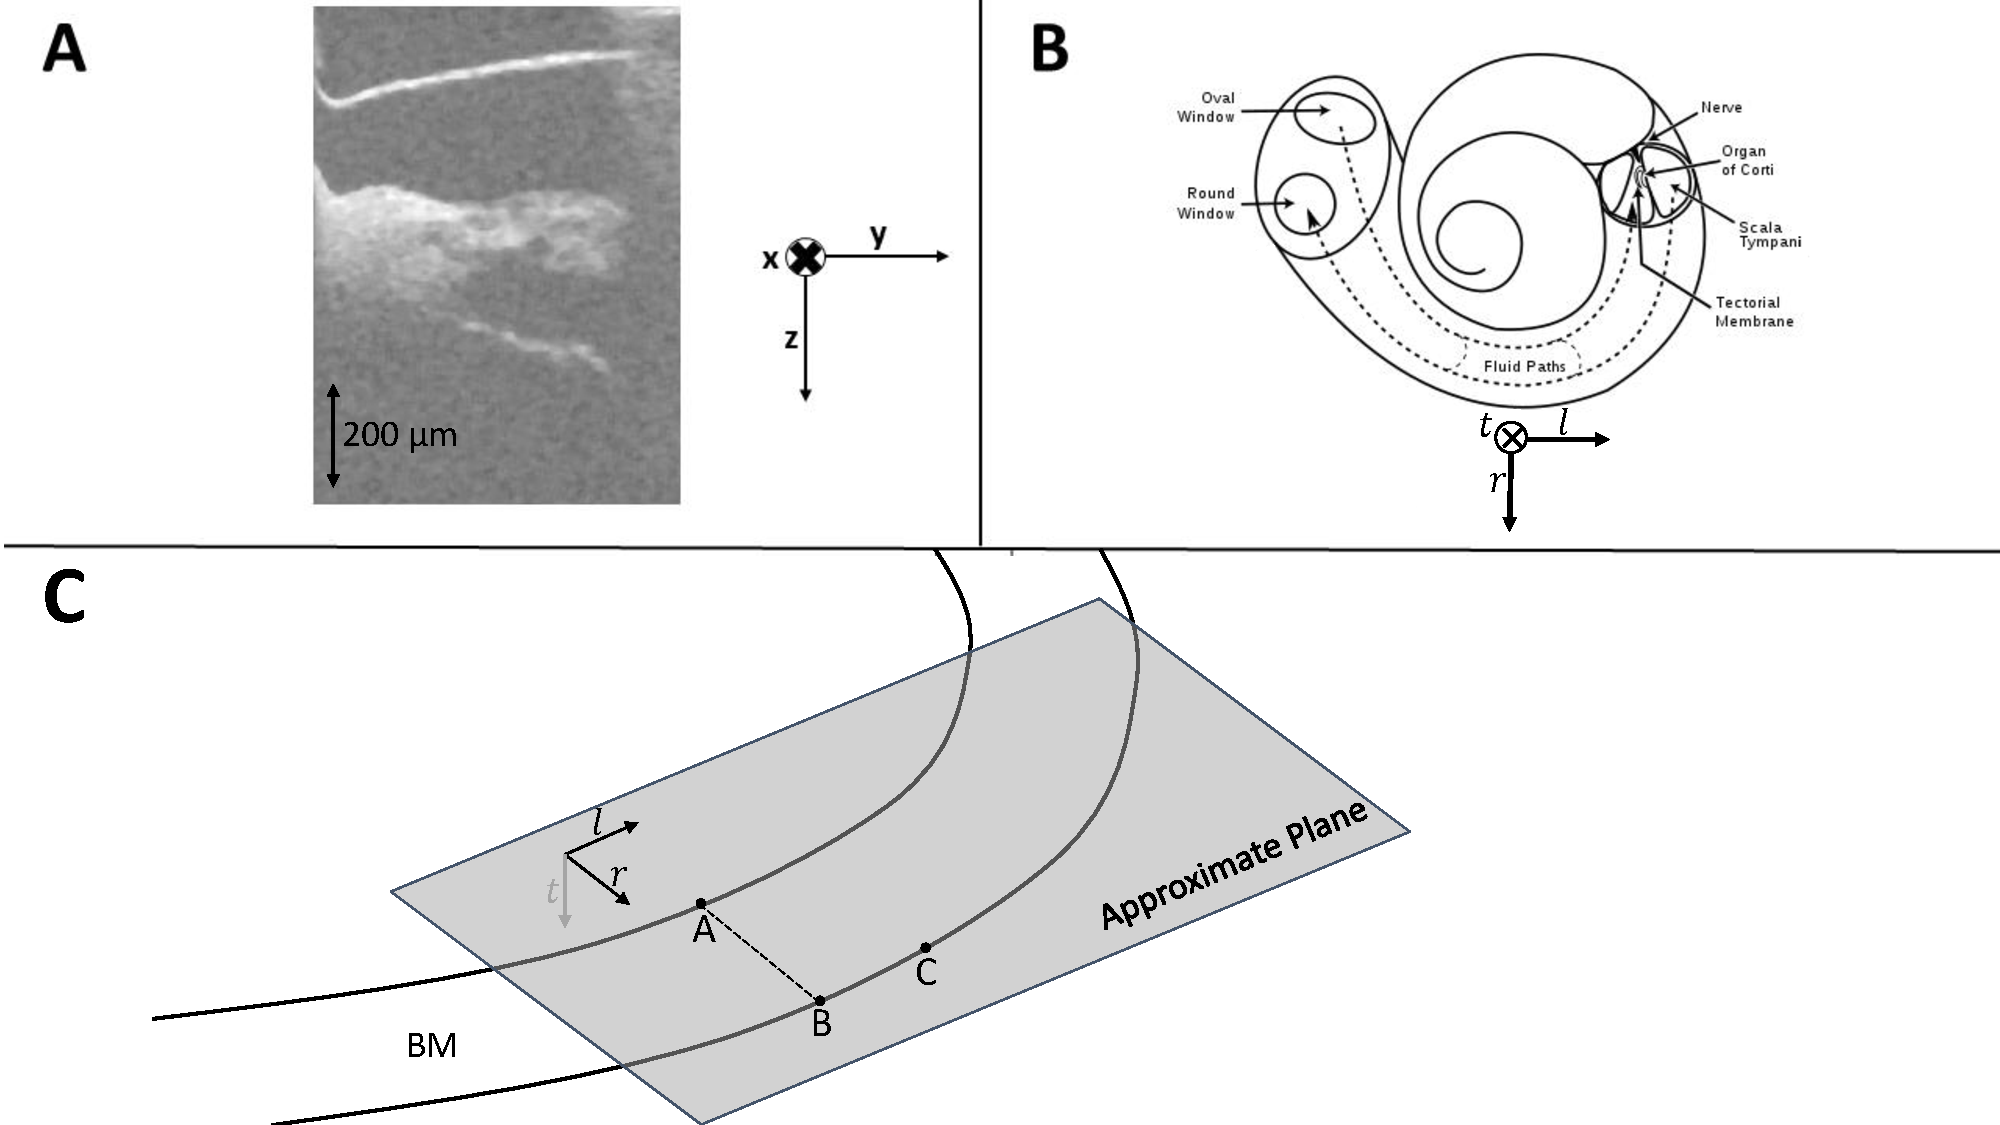
\includegraphics[width=\textwidth]{Figure2.pdf}
\caption{The coordinate systems used in the development of this program. \textbf{A} -- the optical coordinate system, defined with respect to the orienting B-Scan, shown alongside a representative B-Scan; \textbf{B} -- the anatomical coordinate frame, which varies so as to always be tangent to the BM at any point, shown at a point along a cartoon of the cochlea; \textbf{C} -- the local approximation of the anatomical coordinate system, defined with respect to a plane that approximates the BM's plane (shown as a gray surface).}
\label{coords}
\end{figure}

\clearpage
\bibliography{mybib.bib}

\end{document}
